\documentclass[a4paper,12pt]{article}

\usepackage[russian]{babel}
\usepackage{cmap}
\usepackage[utf8]{inputenc}
\usepackage[usenames]{color}
\usepackage{tabularray}
\usepackage{xcolor}
\usepackage{graphicx} 
\usepackage{subfigure}
\usepackage{subcaption}

\usepackage[unicode]{hyperref} % цвета гиперссылок
\hypersetup{
	colorlinks,
	citecolor=black,
	filecolor=black,
	linkcolor=blue,
	urlcolor=black
}

\usepackage{geometry} % задаёт поля 
%\geometry{left=3cm}
%\geometry{right= 1.5cm}
%\geometry{top=2cm}
%\geometry{bottom=2cm} 

\usepackage{enumitem} % настраивает работу со списками:
\def\labelitemi{—} % ... задаёт длинное тире как стандартный маркер ненумерованного списка
\setlist{nolistsep} %  ... убирает дополнительный отступы между элементами списка


% удаляет названия и продолжение следует и т. для таблиц, будет только таблица без всего
\DefTblrTemplate{contfoot-text}{default}{}
\DefTblrTemplate{conthead-text}{default}{}
\DefTblrTemplate{caption}{default}{}
\DefTblrTemplate{conthead}{default}{}
\DefTblrTemplate{capcont}{default}{}


\title{Алгоритмический поиск локтевой точки\\	для определения приемлемых значений\\ метрик машинного обучения }
\author{В. Г. Мосин}
\date{}

%   \input{preamble.tex}
\begin{document}
	\maketitle
	\abstract{\noindent  В статье предложен метод аналитического вычисления локтевой точки для какой-либо метрики машинного обучения, основанный на линеаризации анализируемой метрики и построении ансамбля из двух регрессионных моделей. Изложены теоретические принципы регрессионного ансамблирования, приведен алгоритм поиска локтевой точки по предложенному авторскому методу, рассмотрены примеры работы алгоритма на синтетических данных. }
	
\tableofcontents
	
\section{Введение}
Метрики в машинном обучении — это числовые показатели, которые используются для оценки качества модели или алгоритма машинного обучения. Они помогают понять, насколько хорошо модель работает на конкретной задаче и насколько точно она делает прогнозы. Существует множество различных метрик машинного обучения, которые предназначены для оценки различных моделей (см. [2], [3]).

Например, качество регрессионной модели может оцениваться средней абсолютной ошибкой MAE, средней квадратичной ошибкой MSE или коэффициентом детерминации R2, причем первые две метрики дают хорошую оценку при своих наименьших значениях, близких к 0, а последняя — при своих наибольших значениях, близких к 1. 

Качество кластеризации может оцениваться при помощи таких метрик как индекс Дэвиса-Болдуина,  индекс Рэнда или силуэт, причем первая дает хорошую оценку при наименьших значениях, а последние две — при наибольших. 

Для оценки качества моделей классификации используется множество метрик: процент совпадений, точность, полнота, F1-мера, метрика ROC AUC и т. д. Большинство из них дают хорошую оценку модели при достижении своих наибольших значений, но некоторые — при достижении наименьших.


\subsection{Теоретическая часть}

Можно было бы сказать, что повышение качества какой-либо модели машинного обучения (регрессии, кластеризации или классификации) эквивалентно оптимизации соответствующей метрики, то есть, нахождению таких параметров модели, при которых метрика принимает свое наибольшее или наименьшее значение в зависимости от характера метрики. 

Но это не так.

Хороший пример доставляют регрессионные модели, для которых максимальное значение коэффициента детерминации, равное 1, должно было бы указывать на идеальность модели. Но если какая-либо регрессионная модель демонстрирует такое значение $R^2$, то это однозначно свидетельствует о том, что модель переобучена и вообще не обладает никакой прогнозирующей способностью.

Другой пример — метрика силуэта в кластеризации. Максимальное значение этой метрики равно 1, причем оно никогда не достигается даже теоретически, что, на первый взгляд, выгодно отличает метрику силуэта от коэффициента детерминации. Но для каждого набора объектов есть свой максимум силуэта, и если он достигнут, то это говорит отнюдь не об оптимальной кластеризации, а о том, что все объекты объединены в один кластер.

Поэтому при решении задач машинного обучения, как правило, стремятся привести метрики не к максимальному (минимальному) значению, а к так называемой точке локтя. В литературе эту точку иногда называют точкой сгиба (что неудобно из-из сходства с точкой перегиба), а иногда — точкой перегиба (что вообще не верно). Правильнее всего определить ее как точку, переход через которую уже не приводит к существенному изменению метрики, хотя это не является определением в строгом математическом смысле, так как «существенное изменение» оставляет широкое поле для произвольного толкования.

В качестве иллюстрации этого понятия отошлем читателя к рис. 3 настоящей статьи, где локтевые точки найдены и указаны для синтетических данных. Отметим, что даже если анализируемая кривая является не статистической, а аналитической, локтевая точка это не стационарная точка, не точка экстремума, не точка перегиба и не точка максимальной кривизны. 

\subsection{Постановки задачи}
Когда исследователь применяет метод локтя, его действия состоят в визуальной оценке графика изучаемой метрики. За этими красивыми словами кроется тот факт, что исследователь определяют локтевую точку на глаз. И хотя при этом используются более корректные слова — визуально или интуитивно, сути это не меняет.

\subsubsection{Предмет исследования}

Нами предлагается метод определения локтевой точки, который выполняется автоматически, без учета субъективного мнения исследователя.

\subsubsection{Методика исследования} 

Мы реализуем наш метод в виде алгоритма и применяем его к наборам синтетических данных с различным характером поведения (возрастание, убывание, множественные перегибы и т. д.)

\subsubsection{Цель исследования} 

Наша цель — продемонстрировать, что в большинстве случаев, распространенных в практике применения различных метрик машинного обучения, предложенный нами алгоритм дает приемлемые оценки для определения локтевой точки.

\subsection{Библиотеки}
Для выполнения вычислений и анализа данных мы пользуемся средой \texttt{Jupyter Notebook}, которая предоставляет удобные средства для работы с языком программирования Python и его главными библиотеками: \texttt{NumPy}, \texttt{Pandas}, \texttt{sklearn} и \texttt{matplotlib}. Благодаря этим инструментам, мы можем эффективно работать с данными, выполнять исследования и визуализировать результаты (см. [1], [2]). 

%Библиотека \texttt{numpy} является одной из ключевых библиотек для научных вычислений и обработки массивов данных в языке программирования \texttt{Python}. Библиотека \texttt{pandas}~--- одна из наиболее популярных и мощных библиотек для работы с данными в языке программирования \texttt{Python} (см. [1]). 
%
%Библиотека \texttt{scikit-learn}, широко известная как \texttt{sklearn}, предоставляет обширный набор инструментов и функций для решения различных задач в языке программирования Python, таких как задачи классификации, регрессии, кластеризации и др. Мы используем эту библиотеку для решения регрессионных задач.


\section{Функция \textbf{\texttt{fold\_point}}}

Итак, считается, что локтевую точку нельзя вычислить аналитически. Общепринятая позиция состоит в том, что метод локтя — это эвристический метод, который основан на визуальной оценке графика, и нет точной математической формулы или аналитического метода для определения этой точки. Оценка графика является субъективной и зависит от интуиции и опыта аналитика.

\subsection{Идея алгоритмического определения\\ локтевой точки}

Наша идея состоит в том, чтобы применить ансаблирование регрессионной модели путем линеаризации фрагментов целевой функции, в качестве которой мы будем рассматривать значения анализируемой метрики. Опишем принцип линеаризации, ограничиваясь одномерным случаем, который в дальнейшем и будет для нас актуальным (см. [5], [6]).

Оценка линейной регрессионной модели проводится при помощи коэффициента детерминации $R^2 = 1 - S^*/S’$, где:

\medskip\noindent
\begin{enumerate}
	\item $S^*$ — сумма квадратов отклонений прогнозируемых значений целевой функции от ее истинных значений,
	\item $S’$ — сумма квадратов отклонений истинных значений целевой функции от ее среднего значения.
\end{enumerate}

\medskip\noindent
Если разбить промежуток изменения предиктора на два участка, построить на каждом из них линейную модель и вычислить совокупный коэффициент детерминации для ансамбля из двух моделей, то суммарное отклонение в знаменателе останется точно таким же, но суммарное отклонение в числителе станет меньше (см. рис. 1).

\begin{figure}[!h]
	\centering
	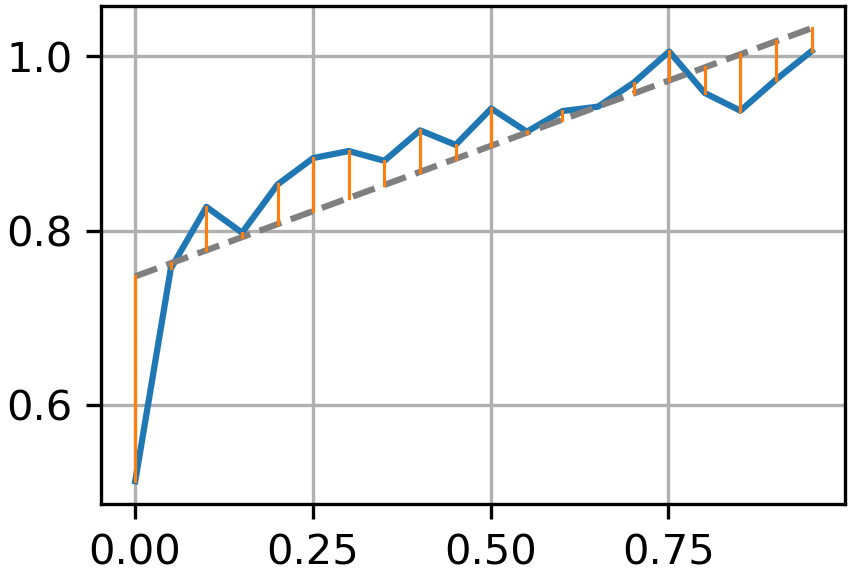
\includegraphics[width=0.4\linewidth]{pictures/Без ансамбля}
	\hspace{0.05\linewidth}
	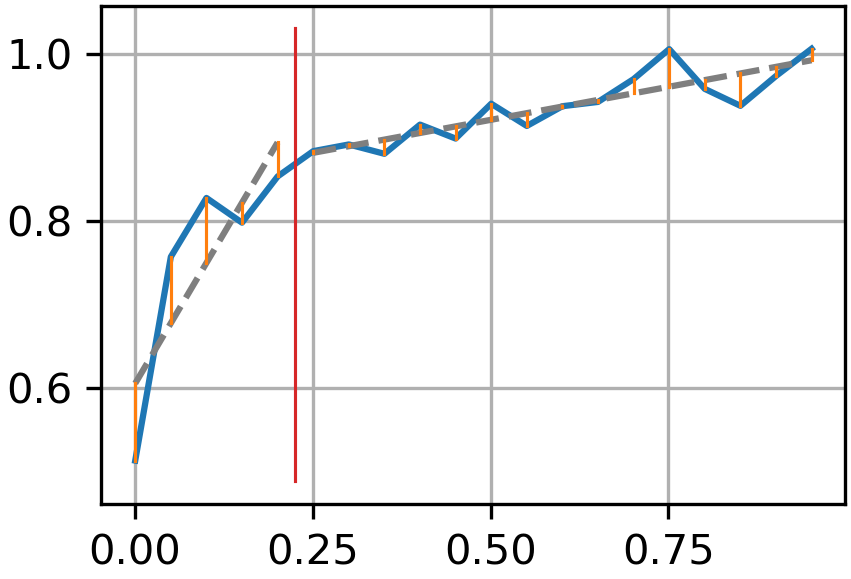
\includegraphics[width=0.4\linewidth]{pictures/С ансамблем}
	\\
	\caption{Линейная модель и ансамбль из двух линейных моделей}
\end{figure}

Это приводит к повышению коэффициента детерминации. 

Теперь допустим, что кривая, которую мы аппроксимируем — это какая-либо метрика машинного обучения (например, метрика силуэта в кластеризации), и мы занимаемся поиском точки локтя для этой кривой. Если осуществить перебор точек разбиения линейной регрессионной модели на ансамбль из двух моделей (см. рис. 2), вычисляя в каждой точке разбиения совокупный коэффициент детерминации, то среди них найдется точка, к которой $R^2$ примет максимальное значение. Это и будет локтевая точка.

\begin{figure}[!h]
	\centering
	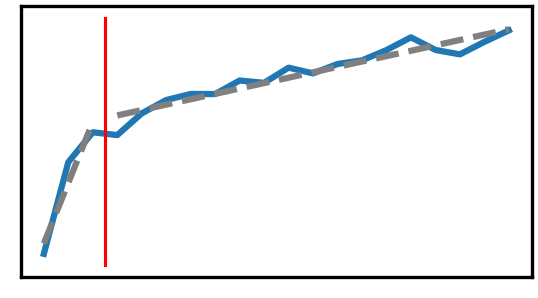
\includegraphics[width=0.25\linewidth]{pictures/1 итерация}
	\hspace{0.01\linewidth}
	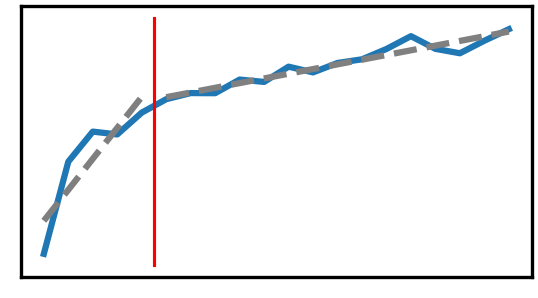
\includegraphics[width=0.25\linewidth]{pictures/2 итерация}
	\hspace{0.01\linewidth}
	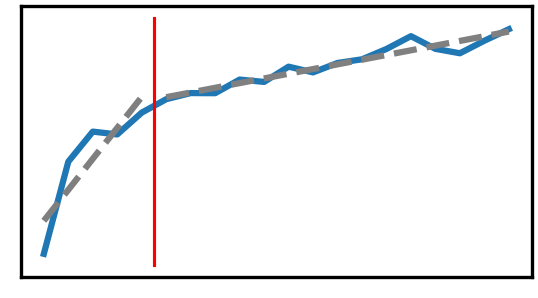
\includegraphics[width=0.25\linewidth]{pictures/2 итерация}
	\\
	\caption{Поиск наилучшей аппроксимации}
\end{figure}
Таким образом, поиск локтевой точки сводится к поиску максимума в списке коэффициентов детерминации, а это сугубо формальный критерий, который никак не апеллирует к опыту и интуиции исследователя и использует аналитические, но никак не визуальные методы поиска.

\subsection{Алгоритм функции \texttt{fold\_point}}
Функция принимает на вход два одномерных массива одинаковой длины, то есть, имеет вид \texttt{fold\_point(A, B)}, где \texttt{A} и \texttt{B} — упомянутые массивы, причем \texttt{A} играет роль независимой горизонтальной переменной, а \texttt{B} является зависимой вертикальной переменной.
В теле функции последовательно выполняются следующие действия.

\subsubsection{Вычисление знаменателя $R^2$}


Напомним, что коэффициент детерминации определяется следующей формулой:
$$
R^2 = 1 - \frac{\displaystyle\sum (y^*_i - y_i)^2}
{\displaystyle\sum (y' - y_i)^2}
$$
где $y_i$~--- истинные значения наблюдаемой характеристики, $y^*_i$~--- предсказанные значения, а $y'$~--- среднее от истинных значений.

При вычислении знаменателя $S’$ используются только сведения о вертикальной переменной (предсказания модели в ней не используются). Так как вертикальную переменную мы уже получили на входе (это массив \texttt{B}), мы сразу же при помощи стандартных функций библиотеки \texttt{numpy} вычисляем \texttt{((B.mean() - B)**2).sum()} и записываем полученное значение в переменную \texttt{S\_line}.


\subsubsection{Пустой список коэффициентов детерминации} 

Создаем список \texttt{R2\_list}, в который будем заносить найденные в ходе работы функции коэффициенты детерминации, и на старте работы функции, еще до исполнения цикла, присваиваем ему значение пустого списка.

\subsubsection{Установка сдвига}

Одномерная задача линейной регрессии имеет смысл, начиная с трех точек (так как прямая проходит через две точки). Поэтому и левый, и правый участок разбиения горизонтальной переменной должны иметь длину, не меньше, чем три позиции. Исходя из этих соображений, объявляем переменную \texttt{shift=3}. Именно таков будет отступ и слева, и справа при исполнении цикла.

\subsubsection{Стартовое значение счетчика цикла} 

Заводим счетчик цикла \texttt{i}, который будет изменяться в пределах длины массива \texttt{len(A)} с отступами на величину \texttt{shift} слева и справа. На старте цикла присваиваем счетчику значение \texttt{i=shift}.


\subsubsection{Данные для левой регрессии}

Используем срезы массивов \texttt{A[:i]} и \texttt{B[:i]} и формируем: 

\medskip\noindent
\begin{enumerate}
	\item предиктор \texttt{X\_left = A[:i].reshape(-1, 1)};
	\item целевую функцию \texttt{y\_left = B[:i]}
\end{enumerate}

\medskip\noindent
для регрессионной задачи на левом участке разбиения.

\subsubsection{Обучение левой регрессионной модели} 

Используя метод \texttt{LinearRegression(}) из модуля \texttt{linear\_model} библиотеки sklearn, создаем модель \texttt{model\_left}. При помощи метода \texttt{fit} обучаем ее на паре \texttt{(X\_left, y\_left)}.

\subsubsection{Прогноз левой регрессионной модели}

При помощи метода \texttt{predict}, примененного к предиктору \texttt{X\_left}, получаем массив предсказанных значений \texttt{y\_pred\_left}, которые дает левая регрессионная модель.


\subsubsection{Левый фрагмент суммы $S^*$}

Вычисляем сумму квадратов отклонения предсказанных левой моделью значений y\_pred\_left от истинных значений y\_left и результат записываем в переменную S\_star\_left:

\medskip\noindent
\texttt{S\_star\_left = ((y\_pred\_left - y\_left)**2).sum()}


\subsubsection{Правый фрагмент суммы $S^*$}

Так же как и выше, используя другие срезы массивов A[i:] и B[i:], формируем: 

\medskip\noindent

\begin{enumerate}
	\item предиктор \texttt{X\_right = A[i:].reshape(-1, 1)};
	\item целевую функцию \texttt{y\_right = B[i:]}
\end{enumerate}


\medskip\noindent
для регрессионной задачи на правом участке разбиения. После этого повторяем действия  и получаем в итоге правый фрагмент суммы $S^*$:

\medskip\noindent
\texttt{S\_star\_right = ((y\_pred\_right - y\_right)**2).sum()}


\subsubsection{Сумма $S^*$}

Общее значение числителя в формуле для коэффициента детерминации получаем, складывая левый и правый фрагменты:

\medskip\noindent
\texttt{S\_star = S\_star\_left + S\_star\_right}

\subsubsection{Пополнение списка \texttt{R2\_list}}

Вычисляем коэффициент детерминации, пользуясь его определением:

\medskip\noindent
\texttt{R2 = 1 - S\_star/S\_line}

\medskip\noindent
и при помощи метода \texttt{append} заносим найденное значение в список \texttt{R2\_list}. В результате первой итерации цикла в этом списке возникает первое значение.

\subsubsection{Цикл по горизонтальной переменной} 

Увеличиваем значение счетчика на 1 и повторяем действия до тех пор, пока счетчик не окажется равным длине \texttt{len(A)} массива горизонтальной переменной минус значение сдвига \texttt{shift}. Такое значение для остановки цикла используется, потому что правая регрессионная модель (так же как и левая) должна строиться на промежутке длиной не меньше 3 (см. замечание выше). На выходе из этого цикла получаем список \texttt{R2\_list}, заполненный коэффициентами детерминации для каждого промежуточного значения горизонтальной переменной, по которому производилось разбиение регрессионной задачи на две модели.

\subsubsection{Предварительный индекс локтевой точки}
 
Пользуясь методом \texttt{argmax} библиотеки \textbf{numpy}, получаем индекс максимального значения в массиве \texttt{np.array(R2\_list)}. Но это не индекс локтевой точки в массиве горизонтальной переменной \texttt{A}, потому что нумерация списка \texttt{R2\_list} отличается от списка \texttt{A} на величину сдвига. Поэтому мы дополнительно производим смещение индекса на \texttt{shift} и получаем:


\medskip\noindent
\texttt{fold\_inedex\_draft = np.array(R2\_list).argmax() + shift}


\subsubsection{Индекс локтевой точки}

Найденное на предыдущем шаге значение \texttt{fold\_inedex\_draft} можно было бы считать окончательным (и в ряде случаев это вполне уместно), но есть соображения, позволяющие его уточнить. Эти соображения относятся к конкретной метрике, по отношению к которой мы собираемся применять метод локтя. В настоящей работе мы будем использовать метрику силуэта, которая изменяется в пределах от –1 до 1, и чем выше ее значение, тем кластеризация считается лучше. В силу того, что горизонтальная переменная A задана дискретным набором значений, найденное предварительное значение индекса локтевой точки задает не точку на горизонтальной оси, а промежуток с левой границей \texttt{A[fold\_inedex\_draft - 1]} и правой границей \texttt{A[fold\_inedex\_draft]}. Вертикальная переменная при таких значениях индекса, скорее всего, принимает разные значения, и, в силу сделанного выше замечания о метрике силуэта, нам выгоднее использовать индекс, при котором вертикальная переменная больше. Заметим, что если бы мы ориентировались на какую-либо метрику, для которой меньшее значение является лучшим (например, на среднеквадратичную ошибку), то выгоднее было бы использовать индекс, при котором вертикальная переменная меньше. 

Поэтому для окончательного определения индекса локтевой точки мы применяем дополнительное условие:


\medskip\noindent
\begin{enumerate}
	\item если \texttt{B[fold\_inedex\_draft] >= B[fold\_inedex\_draft - 1]} то в качестве окончательного значения индекса \texttt{fold\_index} мы назначаем найденное выше значение \texttt{fold\_inedex\_draft},
	\item в противном случае \texttt{fold\_index = fold\_inedex\_draft – 1}.
\end{enumerate}

\subsubsection{Выход функции \texttt{fold\_point}}

Функция возвращает номер горизонтальной переменной \texttt{fold\_index}, при котором наблюдается локтевой сгиб.


\subsection{Применение к синтетическим данным}

Для иллюстрации работы функции, определяющей точку локтя, мы генерируем два образца синтетических данных. В качестве горизонтальной переменной мы используем равномерный массив от 0 до 1 с шагом 0.05. Вертикальную переменную строим искусственно: в первом случае это функция, выпуклая вверх, во втором — выпуклая вниз; на обе функции наложен небольшой случайный шум (см. рис. 3).

\begin{figure}[!h]
	\centering
	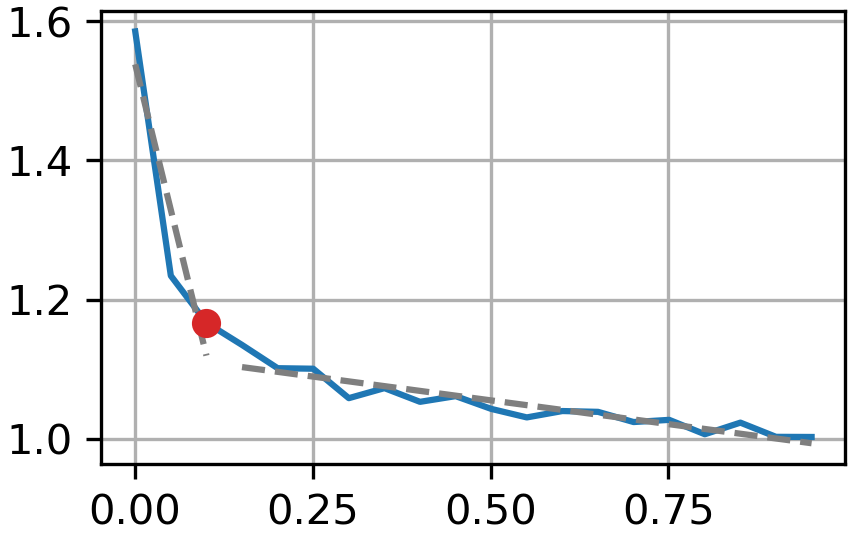
\includegraphics[width=0.4\linewidth]{pictures/Локоть слева}
	\hspace{0.05\linewidth}
	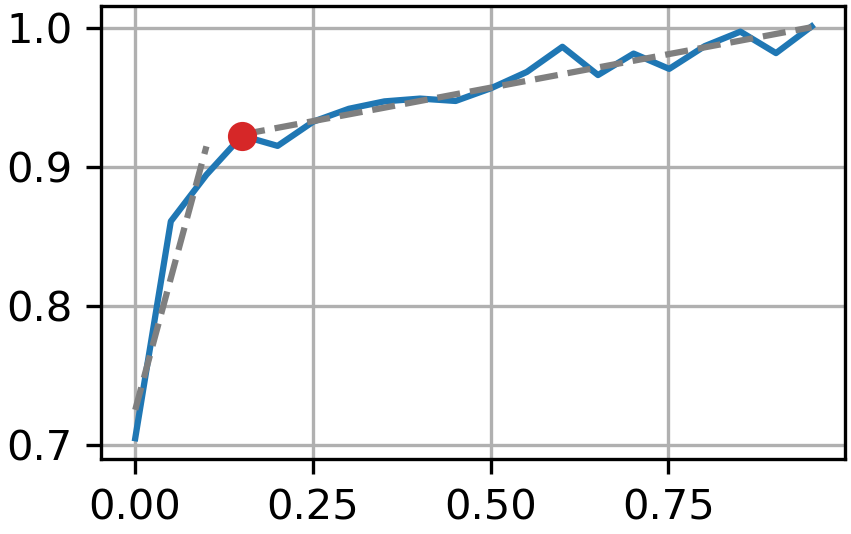
\includegraphics[width=0.4\linewidth]{pictures/Локоть справа}\\
	\caption{Выбор левого или правого значения для индекса}
\end{figure}

Здесь проявляется эффект уточнения индекса локтевой точки. Алгоритм функции \texttt{fold\_point}  определяет не буквальную точку в математическом смысле, а интервал, который своей левой границей задает правую границу левой регрессии, а правой границей — левую границу правой регрессии. И поскольку мы ориентируемся на большее значение метрики, в первом случае в качестве индекса точки локтя выбирается левая граница этого интервала, а во втором случае — правая.


\section{Выводы}

Предложенный метод поиска локтевой точки позволяет избавиться от субъективных суждений исследователя и проводить поиск в автоматическом режиме. Множественные компьютерные эксперименты на синтетических данных показали, что в большинстве случаев, когда исследуемый набор значений действительно обладает локтевой точкой, она удовлетворительно обнаруживается. Это не означает, что в каждом конкретном найденная за счет нашего алгоритма точка действительно является лучшей из возможных локтевых точек. Но в ситуациях, когда поиск локтевых точек должен проводиться многократно и/или в режиме реального времени, предложенный нами метод гарантирует отсутствие грубых ошибок. В целом, изложенный выше алгоритм можно рекомендовать в качестве альтернативы интуитивным методам поиска локтевых точек.

\section{Литература}

\begin{enumerate}
	\item Хейдт М. Изучаем Pandas / М. Хейдт;  — Москва: ДМК Пресс, 2018. — 438 с
	\item Бурков А. Машинное обучение без лишних слов / А. Бурков;  — СПб: Питер, 2020. — 192 с. 
	\item Вьюгин, В. В. Математические основы теории машинного обучения и прогнозирования / В. В. Вьюгин; — М.: МЦИМО. — 2013. — 387~с.
	\item Бринк Х. Машинное обучение / Х. Бринк, Дж. Ричардс, М. Феверолф  — СПб.: Питер, 2017. — 336 с.
	\item В. Г. Мосин, А. В. Караваев. О некоторых проблемах моделирования измеряемых социально-психологических переменных. Математическое образование в современном мире: теория и практика : сборник статей // Самарский государственный технический университет. Всероссийская научно-методическая конференция с международным участием (28–30 ноября 2022~г; Самара); ред. О. В. Юсупова.~--- Самара, 2022.~--- 175 с.
	\item Мосин В.Г. Линеаризация целевой функции в регрессионных задачах методом сингулярных разложений // В книге: Математическое моделирование. Тезисы II Международной конференции. Москва, 2021. С. 66--67.
\end{enumerate}



\end{document}
